\documentclass[conference]{IEEEtran}
%\IEEEoverridecommandlockouts
% The preceding line is only needed to identify funding in the first footnote. If that is unneeded, please comment it out.
\usepackage{cite}
\usepackage{url}
\usepackage{amsmath,amssymb,amsfonts}
\usepackage{algorithmic}
\usepackage{graphicx}
\usepackage{textcomp}
\usepackage{xcolor}
\usepackage{hyperref}
\usepackage{underscore}
\usepackage{setspace}
\usepackage{pdflscape}
\usepackage[export]{adjustbox}
\usepackage{graphicx} %package to manage images
\graphicspath{ {./images/} }
\usepackage[rightcaption]{sidecap}
\usepackage{wrapfig}
\usepackage{caption}
\captionsetup{justification=raggedright,singlelinecheck=false}
\hypersetup{
    colorlinks=true,
    linkcolor=blue,
    filecolor=magenta,      
    urlcolor=cyan,
    pdftitle={Overleaf Example},
    pdfpagemode=FullScreen,
    }
\def\BibTeX{{\rm B\kern-.05em{\sc i\kern-.025em b}\kern-.08em
    T\kern-.1667em\lower.7ex\hbox{E}\kern-.125emX}}
\begin{document}

\title{Hate Speech Detection on Reddit}

\author{\IEEEauthorblockN{Hannah Koizumi}
\IEEEauthorblockA{\textit{School of Data Science} \\
\textit{University of Virginia}\\
Charlottesville, USA\\
hek3bm@virginia.edu}
\and
\IEEEauthorblockN{Anonymous}
\IEEEauthorblockA{\textit{School of Data Science} \\
\textit{University of Virginia}\\
Charlottesville, USA\\
Anonymous@virginia.edu}
\and
\IEEEauthorblockN{Thomas Lever}
\IEEEauthorblockA{\textit{School of Data Science} \\
\textit{University of Virginia}\\
Charlottesville, USA\\
tsl2b@virginia.edu}
\
}

\maketitle

\begin{abstract}
\textbf{The rise in online hate speech over the past 10 years has led most social media companies to update their content policies to explicitly condemn and remove hate speech and ban its perpetrators. However, the constant evolution of hate speech and the tremendous amount of content requiring review are significant barriers to detection. In our experiment, we fine-tuned variants of Bidirectional Encoder Representations from Transformers (BERT) on three labeled hate speech data sets. We then tested these models using Reddit comments posted 72 hours before and after Reddit's major content policy change posted on June 29, 2020. The major content policy change targeted hate speech and other offensive posts. We examined model performance and the limits of these models predicting hate speech in Reddit comments. Qualitative analysis of the test results revealed similarities in hate speech prediction for all but one model that was the only one trained on an augmented balanced dataset.}
\end{abstract}

\begin{IEEEkeywords}
natural language processing, language models, text analysis, language parsing and understanding, neural models, ethical/societal implications, hate speech, Reddit
\end{IEEEkeywords}


\section{Introduction}
The ever-expanding corpus of online hate speech remains a relevant topic of public discourse around free speech and what, if any, responsibility social media companies have to monitor content on their platforms. In the United States, this increase in online hate speech led some social media companies to tighten bans on certain types of speech by changing their user policies. However, one particularly vexing issue remains for United States-based social media ---the lack of a “blanket definition of hate speech under American law, which is generally much more permissive than other countries because of the First Amendment to the US Constitution”\cite{b1}. 

Most major social media platforms have banned hate speech and use automated hate speech detection\cite{b2}. For example, in 2017, Twitter implemented new policies to remove hateful and abusive speech from their platform\cite{b3}; however, research showed an increase in hate speech on Twitter (now X) after Elon Musk purchased the company\cite{b1}. In 2020, Reddit updated their content policy in an attempt to discourage inappropriate speech, specifically citing the desire to reduce hate speech\cite{b4}. It is this shift in policy that is the basis of our project ---identifying online hate speech.

Complicating online moderation of hate speech is algospeak. Algospeak rose as “... a communicative practice in reaction to experiencing content moderation on a platform” and to “circumvent... algorithmic content moderation\cite{b5}. Algospeak is “commonly understood as abbreviating, misspelling, or substituting specific words... when creating a social media post with the particular goal to circumvent a platform’s content moderation systems”\cite{b5}. Algospeak has its roots in a backlash to Google Jigsaw’s Conversation AI, which was introduced in 2016\cite{b6}. The limits of automatic hate speech detection is a challenge. Our research for this project did not specifically identify deep learning models that have been adapted to understand algospeak.

To support our project, we reviewed scholarly literature related to the detection of online hate speech through deep learning methods. We also identified a source for labeled hate speech training data and unlabeled Reddit testing data to be used in conjunction with pre-trained language models. Our goal was to examine the performance of and possibly improve specific pre-trained hate speech or other Natural Language Processing (NLP) deep learning models on Reddit submissions and comments before and after Reddit made a major content policy change on June 29, 2020.

\section{Motivation}
The motivation behind this project is the belief that deep learning models may have great potential to process and detect hate speech in a large sea of content, likely contaminated with hate speech, leading up to the 2024 United States presidential election. Moderating online content, while respecting the generally recognized First Amendment right to freedom of speech, is and will continue to be one of the greatest challenges of our generation, particularly with the already significant increase in User-Generated Content (UGC) and Artificial Intelligence Generated Content (AIGC).

Our project tries to connect data science with social media policy changes. Through this connection, we may be able to trace the evolution of hate speech on the Reddit platform as users reacted to these changes. This approach offers new perspectives to researchers related to trends in hate and violent speech. Researchers may want to consider these trends when creating new models or updating existing models used to detect hate speech. There is no doubt this type of modeling, including frequent model updates, will be an ongoing need as the online social media landscape constantly adapts and evolves.

\section{Method}

\subsection{Overview}
Our research method capitalized on the robust capabilities of BERT-based binary classifiers, renowned for their effectiveness in natural language understanding tasks since BERT's inception in 2018\cite{b7}. The BERT family is a natural first step because it is a Natural Language Processing (NLP) industry standard and is pre-trained on a large corpus. We trained three BERT family models (BERT, DistilBERT, and TinyBERT) on various combinations of three labeled hate speech datasets to be used in testing unlabeled Reddit comment submissions. 

We initially planned to test all Reddit submissions 30 days prior to and 30 days after June 29, 2020. The size of these data files and computing resource constraints led us to narrow the scope to 72 hours prior to and after the policy change was posted. We tested 100\%\ of the data within this period. The labeled training/validation data sets were downloaded from Kaggle\cite{b8} and Hugging Face\cite{b9}. 

A qualitative analysis of the prediction results was completed because the resulting unsupervised predictions could not be compared to the labeled data used for fine-tuning. However, without knowing the model prediction results, each team member reviewed and manually labeled approximately 1000 submissions as hate speech or not speech. These results were combined with the model predictions for our analysis. Our approach is well supported by the code, data sets, and documentation described on Hugging Face\cite{b9}, GitHub\cite{b10}, and Medium\cite{b11}.

\subsection{Architecture}
Transformers, as used in the BERT-family, overcome Recurrent Neural Network (RNN) model short-term memory loss (vanishing gradient) and build upon Long Short-Term Memory (LSTM) models by moving the attention mechanism outside the RNN. Transformers, as opposed to RNNs, LSTMs, and Convolutional Neural Networks, do not use word position as the reference\cite{b12}. Transformers "replace the recurrent layers most commonly used in encoder-decoder architectures with multi-headed self-attention"\cite{b13}. This structure allows transformers to not only look to the traditional 'right' but also to the 'left' during word embeddings and thus provides a greater context to model learning. Flowing from the transformer model is the BERT model which was the "first deeply bidirectional, unsupervised language representation, pre-trained using only a plain text corpus (in this case,Wikipedia)"\cite{b14}.

The use of BERT as the foundation for sequence classification allows the model to have a deep understanding of language nuances and intricacies, making it highly effective for tasks requiring comprehension of context, such as sentiment analysis or hate speech detection\cite{b15}. BERT family models are trained in two steps: pre-training and fine-tuning. BERT was pre-trained with two tasks: Masked Language Modeling (15\%\ of words masked) and Next Sentence Prediction including the relationship between sentences\cite{b12}.  

For the fine-tuning step, BERT-family models are initialized with the parameters from pre-training. We used the three labeled hate speech datasets to fine-tune the models to our specific requirements. Each model, though pre-trained on the same corpus, is unique due to the fine-tuning specifications\cite{b12}.

TinyBERT and DistilBERT evolve in a slightly different manner. These models use knowledge distillation during the pre-training phase which requires the models to learn the BERT model responses to its pre-training steps rather than pre-training on the corpus itself. This technique allows the models to retain most of BERT's learned knowledge while, because layers are removed, providing a lighter weight, faster resource\cite{b16}. Figure number \ref{fig:model} compares the architecture of our project's three models. Figure number \ref{fig:flow} outlines the basic data flow for the three models.

\section{Experiments}
\subsection{Overview}
Our preliminary experiments weighed heavily on test data acquisition and cleaning followed by model creation, training (fine-tuning the final BERT layer) and validation. One test run was accomplished on a TinyBert model to ensure the test model coding was working. The same test data was run by all models and mainly analyzed using qualitative methods due to the unsupervised testing. Challenges to the test phase included computing resource constraints experienced due to model execution demands and volume of test data. 

\subsection{Acquire and Clean Data}
We sought to identify a source of raw data that encompassed all Reddit submissions and comments. A valid torrent was identified that met this requirement. The torrent files\cite{b17} for June and July 2020 were torrented, uncompressed, uploaded into a Jupyter Notebook and converted to Pandas dataframes. The data were systematically explored and cleaned by removing rows and columns not relevant to our analysis. Removals included null entries, Chinese characters, or submissions and comments that had been removed by Reddit or the submitter. Saving the resulting data frames as a feather file allowed them to be easily shared with the entire team. 

\subsection{Train and Validate}
 Fine-tuning the models on the three large training dataset sources presented resource issues given the constraints experienced by the team. The first attempt with a binary classifier based on the full BERT model with a large training dataset (over 400k rows) revealed the importance of adequate computing memory on local machines. Rivanna and Google Colab environments also initially presented resource issues. Rivanna was finally able to be used to train and validate a full BERT-based hate speech binary classifier.
 
To fine-tune the pre-trained models, we identified three hate speech datasets containing text from both Reddit and Twitter. Two hate speech datasets were available from Kaggle\cite{b8} and one from Intelligent Labs\cite{b9}. Table I provides specific details about the datasets.

\begin{table}[h!]
  \caption{Hate Speech Fine-Tuning Datasets.}
  \label{tab:datasets}
  \centering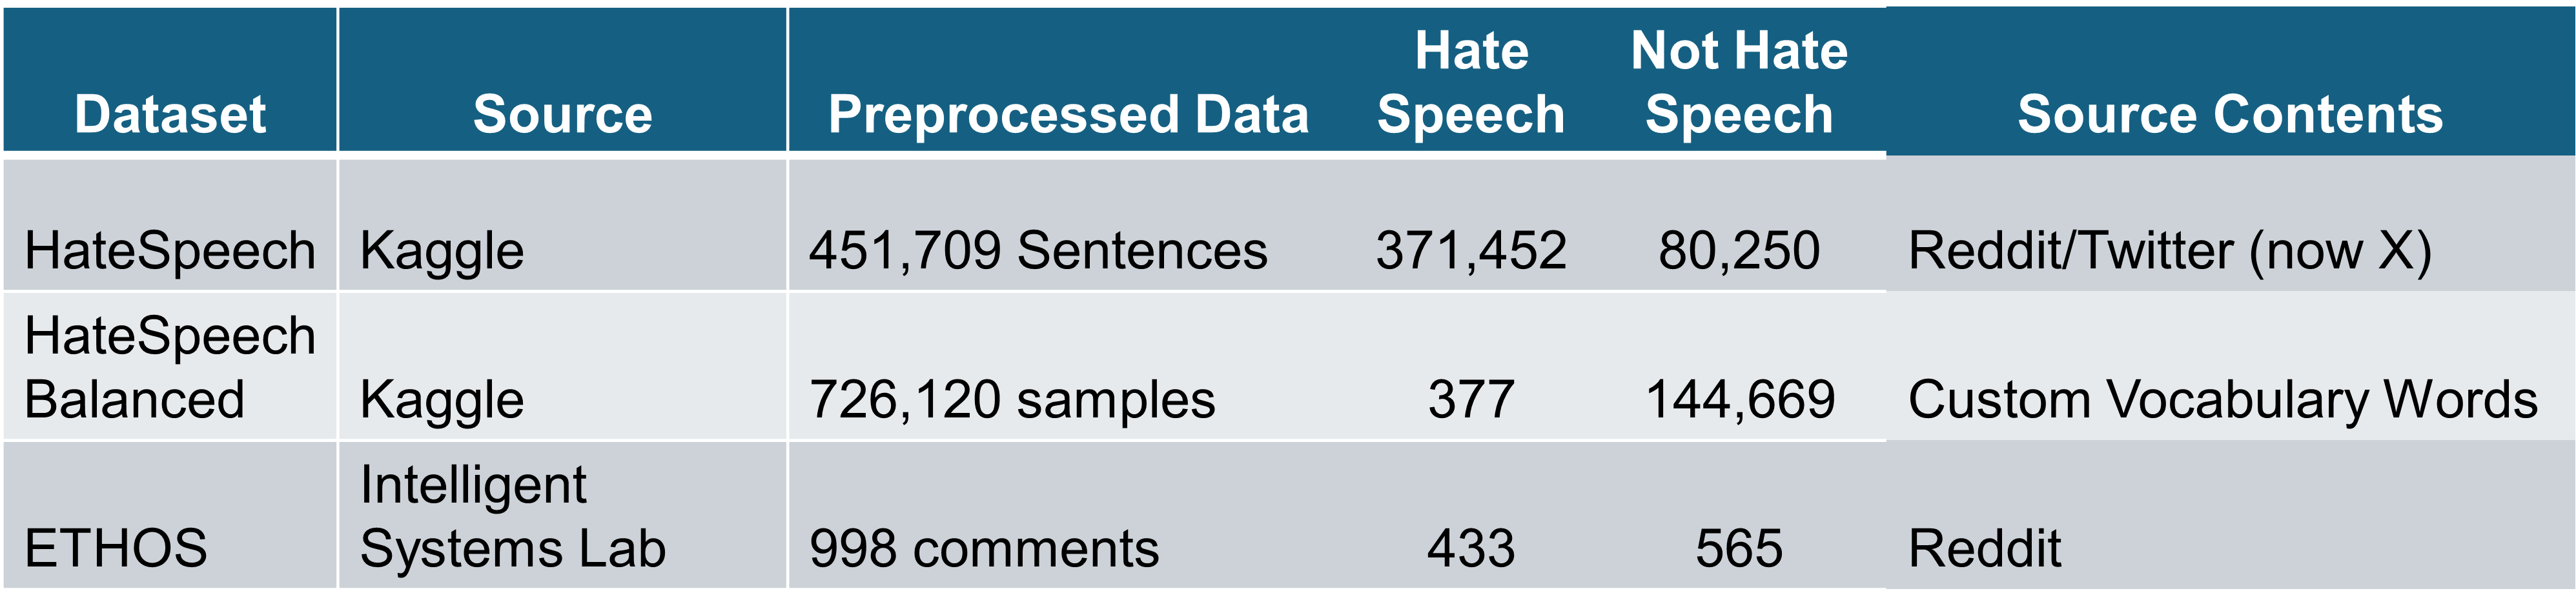
\includegraphics[width=0.5\textwidth]{tabledatasets.png}
  \caption*{Source: Table created by team}
  \caption*{Dataset information: \cite{b8} and \cite{b9}}
\end{table}

\subsection{Fine-Tune Models}
We identified the Hugging Face library\cite{b18} as a reliable source of binary classifier transformer models. We used pre-trained versions of these models which required only fine-tuning the last layer. The first model fine-tuned and tested was BERT which has 12 layers and is  a resource intensive model. Next in line, with 6 layers, was DistilBert --- a lighter weight transformer model that preserves much of BERT's performance\cite{b16}. Lastly, with 2 layers, TinyBert was chosen as one of the lightest footprint models in the BERT family.

In natural language processing (NLP), F1 score is often preferred over accuracy as a measure of model performance, particularly in scenarios where the data exhibits class imbalance. The F1 score balances precision and recall. Precision measures the accuracy of the positive predictions-- the proportion of true positives among all predicted positives, while recall (also known as sensitivity) measures the model's ability to identify all relevant instances-- the proportion of true positives among actual positives\cite{b19}. This balance makes F1 score a more robust performance metric, especially when the cost of false positives differs significantly from false negatives. The F1 score thus provides a more holistic view of a model's performance than accuracy alone, which might be misleading in cases where the majority of the dataset belongs to one class\cite{b19}. The best validation performance for the three models and the three datasets is shown in table II.

\begin{table}[h!]
  \caption{Best Performance Validation.}
  \label{tab:table}
  \centering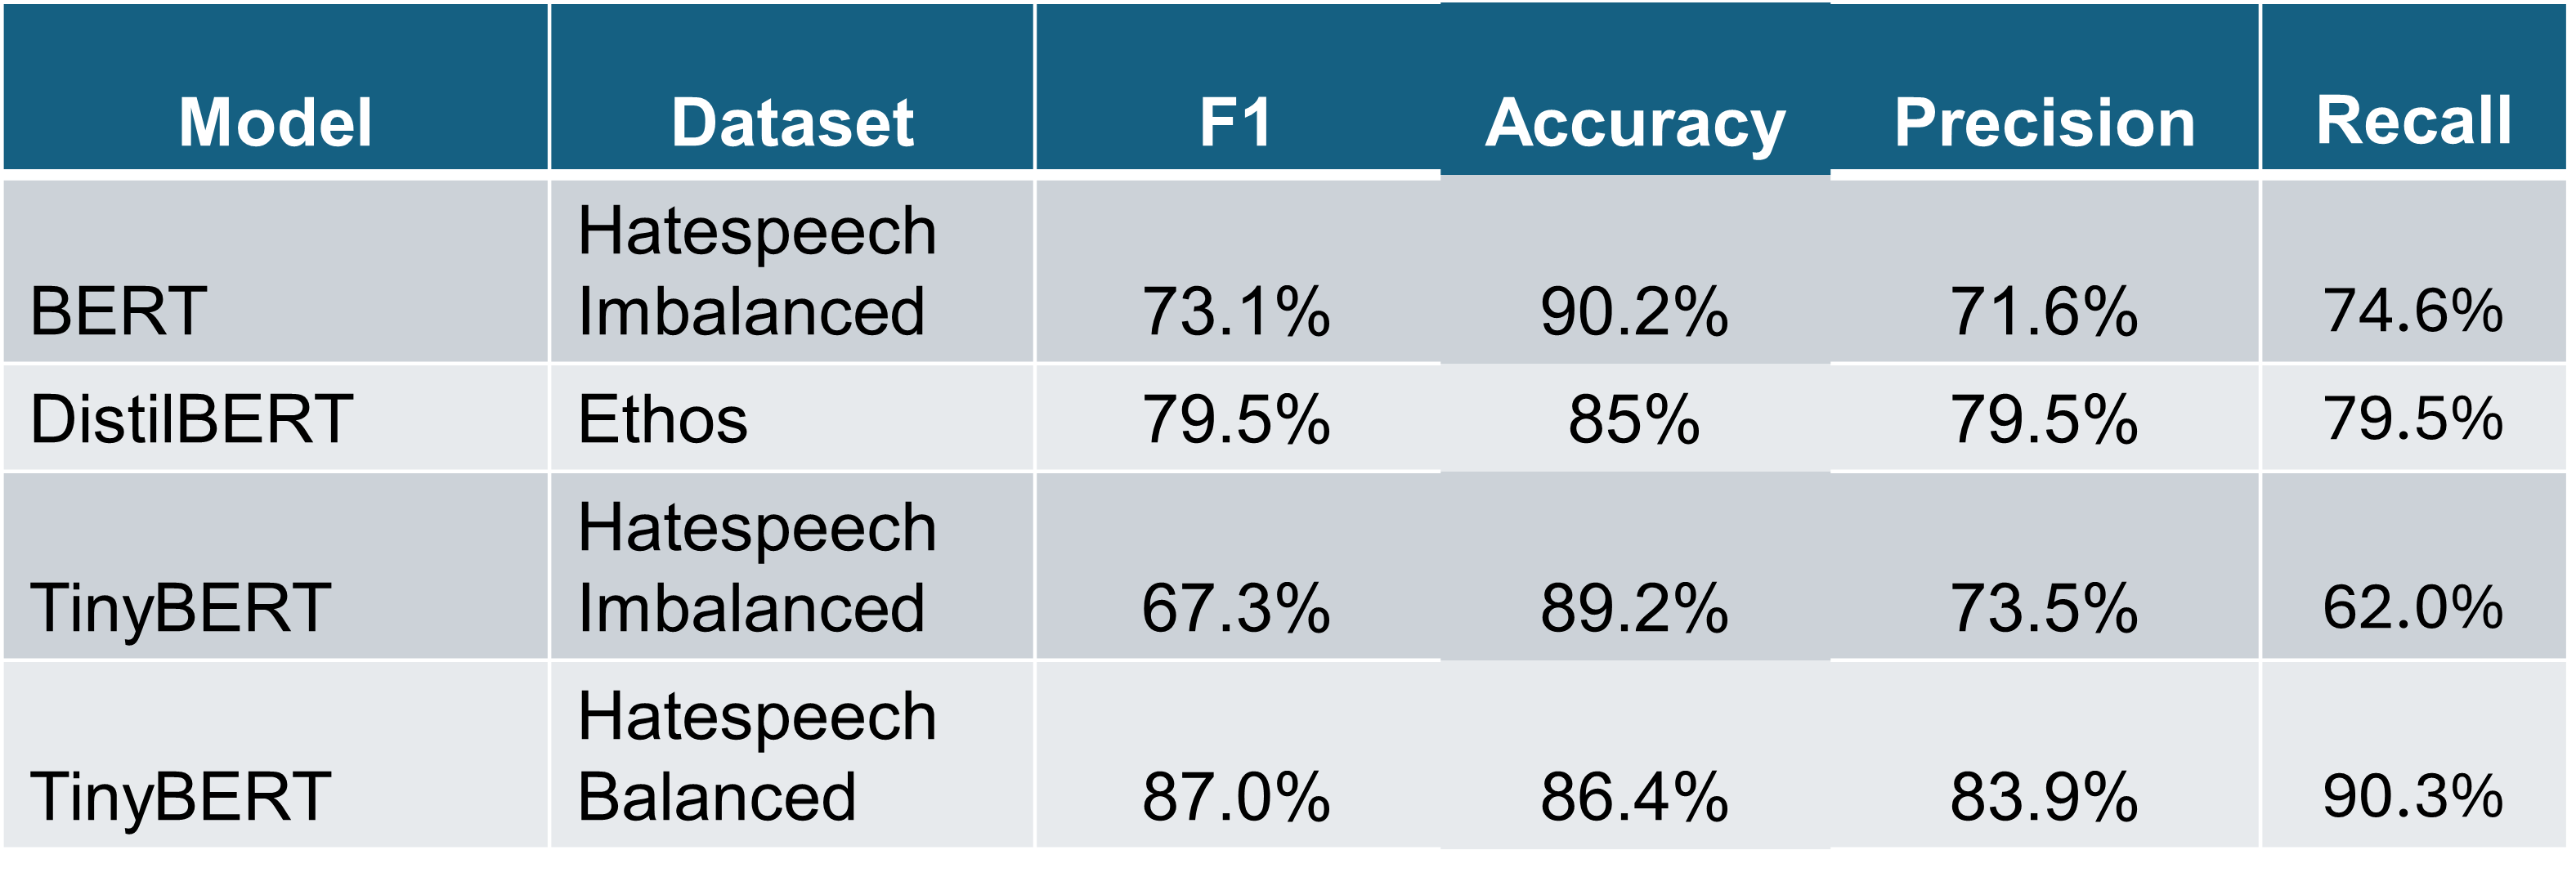
\includegraphics[width=0.5\textwidth]{3.png}
  \caption*{Source: Team Results}
\end{table}

\subsubsection{BERT}
The BERT-based binary classifier, a robust model\cite{b14}, initially presented resource challenges to the team on local machines, Rivanna, and Google Colab. After much effort, the binary classifier was modified to run within Rivanna. The model successfully trained on the imbalanced Hate Speech dataset after setting up checkpoints\cite{b20}. The model was tuned by decreasing the learning rate. Throughout the initial phase of training, involving 3000 backpropagations, the binary classifier model demonstrated promising validation accuracy, with values ranging from 81\%\ to 86.6\%. The best performance validation is shown in table number ~\ref{tab:table}.

\subsubsection{DistilBERT}
The second model, DistilBERT, was chosen because it is a “small, fast, cheap and light Transformer model trained by distilling [the] BERT base. It has 40\%\ less parameters than google-bert/bert-base-uncased, runs 60\%\ faster while preserving over 95\%\ of BERT’s performances as measured on the GLUE language understanding benchmark”\cite{b16}. Despite being lighter weight than the BERT-based classifier, it still tested the boundaries of resources like Google Colab. 

We were able to fine-tune the model, albeit slowly, in the Colab environment. The initial round of training/validation on the ETHOS dataset realized an accuracy of 84\%\ and 78\%\ precision\cite{b21}. The model was tuned by optimizing for F1 instead of accuracy and adjusting the learning rate of the model, the results are shown in table number \ref{tab:table}.

\subsubsection{TinyBert}
TinyBert\cite{b21}, the third model tested, is also a distillation model which has a two-stage learning framework for pre-training as opposed to the single stage learning framework used by distilBERT. Distillation occurs during pre-training, similar to distilBERT and also during the "task-specific learning stages"\cite{b22}. The task specific learning stage, for this project, was the binary classification of two of the three hate speech dataset.  This approach allows TinyBERT, with only 2 layers, to "...capture the general-domain as well as the task-specific knowledge in BERT\cite{b21}. Bhargava, Drozd, and Roger\cite{b23} reported that bert-tiny with 4.4M parameters did not perform worse than bert-medium with 41.7M parameters, showing that more parameters do not necessarily result in better generalization and performance in models.

The TinyBERT model was fine-tuned on both the balanced and imbalanced versions of the hate speech data set.  It is clear that while the imbalanced data, when trained on a few runs, has a higher accuracy rate; the overall results for the balanced dataset show more promise precisely due to it being balanced data. The learning rate hyperparameter is by far the most important (96\%) over batch size for the balanced dataset. Both model results are shown in table number \ref{tab:table}.

\section{Results}
\subsection{Overview}
The initial test run on TinyBERT provided insight into the wide range and varied comments topics in the approximately 1.7M comments in the first days of July 2020. Two histograms show the models' predictions (figure number \ref{fig:histogram}). The prediction difference between the TinyBERT fine-tuned on the balanced dataset and the remaining model/dataset combinations is highly evident and will be discussed below. The test run revealed the top 5 subreddits, in terms of predicted hate speech, on comments published between June 26 and June 27, 2020, were: 1) AskReddit, 2) memes, 3) politics, 4) teenagers and 5) AmItheAsshole. The subreddits figure prominently in the complete test run on both sides of the policy change date. Figure number \ref{fig:top10} shows model predictions for the top 10 subreddits in the before and after policy change data sets. These bar charts also show the same anomaly regarding the balanced TinyBERT model testing. 

Qualitative analysis was used to analyze model test results due to the unsupervised test method. In addition to total test result comparison both before and after, a random sampling of 500 comments before the policy change and 500 after were reviewed by the project team. We hid the model results to avoid bias while labeling our predictions. Figure number \ref{fig:agreement} depicts the total hate speech prediction agreements with other models or team members, again the TinyBERT balanced dateset anomaly presents itself as an outlier. A co-occurrence matrix of hate speech predictions by model and team member present a different perspective on model and team member agreement is shown in figure number \ref{fig:matrix}. 

Time and resource constraints prevented a 100\% review of test results. However, this type of analysis can be useful for an in-depth analysis of why comments are flagged as hate speech by some models and not others or of hate speech entirely missed by all the models. The results may improve how models are created and fine-tuned or how fine-tuning datasets are created and labeled. 

It is expected that hate speech, while pervasive, is difficult to predict in a deep learning environment. Transformers have the benefit of looking left and right, providing the model with wider sentence context. However, the models, as tested, did have the submission (post) and the entire subreddit thread (comments) in one context. Some comments that were predicted to be hate speech were clearly not hate speech, showing the limitations of automated hate speech detection.

\subsection{Model Test Results}
\subsubsection{BERT}
The BERT model performed similarly to the distilBERT and imbalanced TinyBERT in predicting a very small percentage of hate speech among the Reddit comments. Before the Reddit content policy change, 93.35\% of the submissions were predicted as non-hate speech and 6.65\% as hate speech. After the policy change, 93.4\% were predicted as non-hate speech and 6.6\% were hate speech. Out of the three closely grouped models (figure number \ref{fig:histogram}), the BERT model most reliably predicted that comments contained hate speech. Our qualitative analysis found this model was not unique in being able to correctly predict a comment as hate speech. The other tested models also generally identified the comment as hate speech. The few comments in the review sample where BERT predicted a comment as hate speech without corroboration from other models revealed comments that were clearly not hate speech. For example, "that was perfectly executed bravo sir" or "i didnt expect anything else" were Reddit comments identified as hate speech.  These misidentified comments, however, did discuss issues adjacent to or highly correlated with hate speech such as the word "non-binary" or curse words in a non-hate context. 

\subsubsection{DistilBERT}
The DistilBERT model experienced routine kernel crashes when run locally on the test data despite being a lighter weight model than BERT. We were finally able complete model testing in Rivanna. The DistilBERT model used the strictest parameters to predict hate speech, which translated to the lowest percentage of predicted hate speech for both before and after the policy change. Before the policy change, 96.28\% of the comments were predicted as non-hate speech and 3.72\% predicted as hate speech. After the policy change, 96.04\% were identified as non-hate speech and 3.96\% were hate speech. From the qualitative analysis, it was more likely to predict false negatives than false positives given it predicted texts as hate speech relatively infrequently, but there are no other obvious patterns. 

\subsubsection{TinyBERT}
The TinyBERT model trained on the imbalanced data did not differ significantly from the first two models. It predicted 3.86\% of the comments as hate speech before the policy change and 4.21\% after the policy change. The difference between the before and after percentages is larger than the other models. The TinyBERT model trained on the balanced data set had prediction results that significantly deviated from the other four model/dataset combinations as shown in figure number \ref{fig:histogram}. Before the policy change, it identified 57.5\% as non-hate speech and 42.3\% of the data as hate speech. After the policy change, it identified 56.97\% of the data as not hate speech and 43.03\% of the data as hate speech. The balanced dataset was augmented which may have contributed to the anomaly this set presented when testing models.

In reviewing our qualitative analysis, the TinyBERT model trained on the imbalanced dataset performed similarly to the first two models and often agreed with BERT predictions. Of the comments independently labeled as hate speech by our team, this model predicted the most false positives within our sample. TinyBERT trained on the balanced dataset clearly marked things as hate speech that were not even mildly offensive or threatening in any way. Statements like "i didnt expect anything else" or "literally made me cringe" were marked as hate speech. This is the only model that objectively failed at the task of classifying hate speech due to the large amount of false positives.  

Mody, Huang, and deOliveria\cite{b8} provided a profanity file along with their hatespeech\cite{b8} datasets. This file contained what they described as a list of common English profanities, which include words that may or may not be considered hate speech such as vibrator, vulva, butt, and masturbate in conjunction with words always considered hate speech such as honky, kike, spic, and wetback. It is unclear how this list was put together but it is heavily weighted to descriptions of sex and sex acts that may or may not be used in a hate speech context. 

Also, of consideration to the prediction or identification of hate speech is the audience and how the speech relates to the subreddit in which these comments were posted. Online comments may or may not be publicly acceptable speech but this speech may or may not be considered hate speech. The dilemma in ever evolving speech, particularly in informal settings, harkens back to Supreme Court Justice Potter Stewart's comment in 1964's Jacobellis v. Ohio regarding hard-core pornography, "I shall not today attempt further to define the kinds of material I understand to be embraced within that shorthand description, and perhaps I could never succeed in intelligibly doing so. But I know it when I see it, and the motion picture involved in this case [Louis Malle's The Lovers] is not that"\cite{b24}. Certain elements of hate speech are irrevocably hate speech whereas other speech lies within the time and space of evocation. 

\section{Conclusion}
It was unclear, from our testing, whether a visible reduction in hate speech in Reddit comments occurred as a result of the policy change. Reddit banned r/the Donald with a following of 800,000 in this policy change --- the largest pro-Trump community on Reddit. Reddit banned over 2,000 communities as it enforced this content policy change. Steve Huffman, co-founder and CEO of Reddit, discussed the difficulty of balancing political speech with harassing, violent, or bullying speech. Because Reddit was unable to "get that [r/Trump] community to come in line with our content policies"\cite{b25}, it was banned. 

The model predictions realized small differences of predicted hate speech between the two testing datasets (hatespeech imbalanced and ETHOS) with reasonable hate speech predictions. It is plausible that the change in policy has little to no impact in deterring hate speech on Reddit. It is also true that online hate speech has and continues to evolve (algospeak) to avoid content moderation. 

One positive indication may be that the models (except TinyBERT balanced) predicted roughly the same amount of hate speech before and after the policy change. This result may be because the models were robust enough to include evolutionary changes in speech due to the policy change. Although we are not able to draw conclusions about effect of the policy change, the primary purpose of this analysis, we are able to draw conclusions about the methodology of predicting hate speech through deep learning. 

Predicting hate speech with deep learning is not yet nor likely ever be a task with globally approved standards. Without understanding the specific subreddit community and evaluation of the subreddit submission combined with the subsequent thread comments, context is a moving target. The line can be quite thin and fuzzy between crass remarks and hate speech. One encouraging observation from our qualitative analysis was that clear cut examples of hate speech were predicted as such by all models. 

One conclusion from this project is that multiple models may be a tactic when filtering through submissions and comments. A joint model consensus could identify and remove the most heinous comments. This approach could be impossibly resource intensive today but the future could portend this approach as feasible. The resource limitations we experienced during our project are reflective of the real world, computing resources and time make it very difficult to quickly identify and remove online hate speech. The human in the loop with regard to content moderation is still a vital piece of this process --- and continues to be the real reality check.

Our method may be a useful addition to the existing literature on hate speech identification due to the lack of reproducibility and testing on real-world data we found in our literature review. The use of other models and hate speech training data could contribute to our results and increase the understanding of model performance in online content moderation.

Lastly is a discussion of the implications of this project to the well being of Virginia residents. Hate speech is pervasive and to no surprise, is pervasive in online college communities. One study found that college subreddits show a 25\% greater incidence of hate speech than non-college subreddits\cite{b26} Another recent (2023) study discusses the use of artificial intelligence and machine learning approaches to mitigate online hate speech but also discusses the problems we discussed in this report including the rise of algospeak to get around moderation and this issue of context\cite{b27} ---is it hate speech or not? 

The well being of Virginia residents lies within its communities whether in person or online. Increased focus on development of models that will realistically predict hate speech may not be around the next corner, but these models, if they can be developed to be valid, reliable, without bias and without limiting our First Amendment Rights (however they will be defined), may increase the well being of Virginia's residents. 


\section{Team Member Contributions}

\subsection{Thomas Lever Contributions}

\begin{itemize}
  \item Prepared from the Reddit API data from Reddit
  \item Coded for training and validation
  \item Tuned, trained, validated, and tested a hate speech binary classifier using AutoModelForSequenceClassification, bert-base-uncased, and HateSpeechDataset.csv
  \item Assisted team member by testing DistilBERT model in Rivanna using a GPU
  \item Reviewed and labeled about 1000 predictions for qualitative review of test results.
 \item Edited “Identifying Online Hate Speech: Literature Review and Project Proposal"
 \item Completed first draft of Milestone II submission and edited drafts of Milestone II and Milestone III submissions
 \item Asked questions of other groups and provided personal responses to questions to our group during Milestone I presentation
 \item Edited the slideshow presentation
\end{itemize}

\subsection{Hannah Koizumi Contributions}

\begin{itemize}
  \item Set up weekly meetings on Zoom/Set up project Teams channel \&\ Refined idea for NLP project
  \item Identified 2 recent and relevant labeled hate speech training data sets and BERT model
  \item Coded for training and validating datasets
  \item Trained and tuned DistilBERT model on local machine 
  \item Researched and compiled extensive Literature Review
  \item Drafted \&\ edited Milestone I Literature Review and Project Proposal in Word and Overleaf 
  \item Edited and reviewed Milestone II drafts in Word and Overleaf
  \item Co-presented Milestone I presentation
  \item Drafted questions for Milestone I group presentations and answered this group's questions posed by other teams
  \item Drafted \&\ edited Milestone III in Overleaf
  \item Performed qualitative analysis and independent labeling of the 1,000 samples 
  \item Edited the slideshow presentation 
\end{itemize}

\subsection{Anonymous Contributions}

\begin{itemize}
   \item Provided additional research for Literature Review
   \item Identified ETHOS dataset as another training set option
   \item Provided team with model code for DistilBERT and TinyBERT 
   \item Coded Reddit API using \href{https://praw.readthedocs.io/en/stable/}{PRAW} to gather data 
   \item Identified and torrented data for unlabeled Reddit test set
   \item Processed torrent data, loaded into dataframes, stored for team use
   \item Cleaned data to ready for tokenization in the BERT models
   \item Identified DistilBERT \&\ TinyBERT models as options to BERT, coded for training and validating datasets 
   \item On TinyBERT, tuned both hate speech datasets, coded and ran model testing on local machine
   \item Created test code for all models; provided to team
   \item Drafted, edited and reviewed Milestone I, II \&\ III drafts in Word \&\ Overleaf 
   \item Created final versions of Milestone I, II and III and submitted in Canvas for team 
   \item Created Milestone I \&\ III presentations and co-presented  
   \item Merged all prediction results (including team member predictions) for analysis; created before and after random samples
   \item Labeled 1000 random samples in qualitative review
   \item Created all visualizations used in the Milestone III presentation and report
 \end{itemize}

\begin{thebibliography}{00}

\bibitem{b1}"The Musk bump: quantifying the rise in hate speech under Elon Musk." Center for Countering Digital Hate. \href{https://counterhate.com/blog/the-musk-bump-quantifying-the-rise-in-hate-speech-under-elon-musk}{https://counterhate.com/blog/the-musk-bump-quantifying-the-rise-in-hate-speech-under-elon-musk/} (accessed March 7, 2024).
\bibitem{b2}F. Nascimento, G. Cavalcanti, and M. Da Costa-Abrue. “Exploring automatic hate speech detection on social media: a focus on content-based analysis.", vol 13, iss 2, 2023. \href{https://doi.org/10.1177/21582440231181311}{https://doi.org/10.1177/21582440231181311} (accessed March 8, 2024).
\bibitem{b3}D. Lee. “Twitter's hate speech rules are expanded.” BBC. \href{https://www.bbc.com/news/technology-42376546}{https://www.bbc.com/news/technology-42376546} (accessed March 7, 2024).
\bibitem{b4} “Reddit content policy.” Reddit. \href{https://www.redditinc.com/policies/content-policy}{https://www.redditinc.com/policies/content-policy} (accessed March 5, 2024).
\bibitem{b5}E. Steen, K. Yurechko, and D. Klug. "You can (not) say what you want: using algospeak to contest and evade algorithmic content moderation on TikTok. Social Media + Society, vol 9, iss 3, 2023. \href{https://doi.org/10.1177/20563051231194586}{https://doi.org/10.1177/20563051231194586} (accessed March7, 2024).
\bibitem{b6}A. Greenberg. "Inside Google’s internet justice league and its AI-powered war on trolls.", Wired, September 19, 2016. https://www.wired.com/2016/09/inside-googles-internet-justice-league-ai-powered-war-trolls/ (accessed March 8, 2024).
\bibitem{b7} B. Muller. "BERT 101 state of the art NLP model explained.", Hugging Face, March 2, 2022. \href{https://huggingface.co/blog/bert-101}{https://huggingface.co/blog/bert-101}(accessed April 27, 2024).
\bibitem{b8} D. Mody, Y. Huang, and T. deOliveria. "A curated dataset for hate speech detection on social media text.", Data in Brief, vol 46, February 2023. \href{https://www.sciencedirect.com/science/article/pii/S2352340922010356?via%3Dihub} (accessed March 10, 2024).
\bibitem{b9} I. Mollas, Z. Chrysopooulou, S. Karlos, and G. Tsoumakas. "ETHOS: an online hate speech detection dataset.", Complex \&\ Intelligent Systems, vol 8, pp. 4663-4678, January 4, 2022. \href{https://arxiv.org/pdf/2006.08328.pdf} (accessed March 15, 2024).
\bibitem{b10}J. Devlin. Google Research BERT Github, \href{https://github.com/google-research/bert}{https://github.com/google-research/bert} (accessed March 15, 2024).
\bibitem{b11} P. Dholaykia. "Twitter hate detection using: HuggingFace BERT fine-tuning.", Medium, February 10, 2023. \href{https://medium.com/@parthdholakiya180/twitter-hate-detection-using-bert-e7682b2d0a0c}{https://medium.com/@parthdholakiya180/twitter-hate-detection-using-bert-e7682b2d0a0c} (accessed March 24, 2024).
\bibitem{b12} R.Evtimov, M. Falli, and A. Maiwald. "Anti social online behaviour detection with BERT.", Information Systems Seminar (WS19/20), February 7, 2020. \href{https://humboldt-wi.github.io/blog/research/information_systems_1920/bert_blog_post/#}{Bidirectional Encoder Representations from Transformers (BERT)} (accessed April 15, 2024).
\bibitem{b13} A. Vaswani \textit{et al}. "Attention is all you need.", Advances in Neural Information Processing Systems, 2017. \href{https://proceedings.neurips.cc/paper_files/paper/2017/hash/3f5ee243547dee91fbd053c1c4a845aa-Abstract.html}{https://proceedings.neurips.cc/paper_files/paper/2017/hash/3f5ee243547dee91fbd053c1c4a845aa-Abstract.html} (accessed April 14, 2024).
\bibitem{b14} J. Devlin and M.W. Chang. "Open sourcing BERT: state-of-the-art pre-training for natural language processing.", Google Research, November 2, 2018. \href{https://research.google/blog/open-sourcing-bert-state-of-the-art-pre-training-for-natural-language-processing/}{https://research.google/blog/open-sourcing-bert-state-of-the-art-pre-training-for-natural-language-processing/} (accessed April 14, 2024). 
\bibitem{b15} R. Horev. "BERT Explained: State of the art language model for NLP.", Medium, November 10, 2018. https://towardsdatascience.com/bert-explained-state-of-the-art-language-model-for-nlp-f8b21a9b6270 (accessed April 27, 2024).
\bibitem{b16}V. Sanh, L. Debut, J. Chaumond, and T. Wolf. "DistilBERT, a distilled version of BERT: smaller, faster, cheaper and lighter.", March 1, 2020. \href{https://arxiv.org/abs/1910.01108}{https://arxiv.org/abs/1910.01108} (accessed March 20, 2024). 
\bibitem{b17} stuck_in_the_matrix, Watchful1, and RaiderBDev. "Reddit comments/submissions 2005-06 to 2023-12.", \href{https://academictorrents.com/details/9c263fc85366c1ef8f5bb9da0203f4c8c8db75f4}{https://academictorrents.com/details/9c263fc85366c1ef8f5bb9da0203f4c8c8db75f4} (accessed March 8, 2024).
\bibitem{b18} "Transformers".\href{https://huggingface.co/docs/transformers/index}{https://huggingface.co/docs/transformers/index} (accessed March 29, 2024).
\bibitem{b19} J. K. "The F1 score.", Medium, August 31, 2021. \href{https://towardsdatascience.com/the-f1-score-bec2bbc38aa6}{https://towardsdatascience.com/the-f1-score-bec2bbc38aa6} (accessed April 27, 2024).
\bibitem{b20} T. Lever. Hatespeech Binary Classifier Github Repository., \href{https://github.com/tslever/Hate_Speech_Binary_Classifier}{https://github.com/tslever/Hate_Speech_Binary_Classifier} (accessed March 31, 2024).
\bibitem{b21} DS 6050 Teams Channel, \href{https://myuva.sharepoint.com/:f:/s/DeepLearningProject197/Et06vD0Kl0xJtcE_D2ZOK1gB96t8YuGoZFToUYcM4qPz2A?e=e8TSxx}{Teams Channel} (accessed March 31, 2024).
\bibitem{b22}X.Jiao \textit{et al}."TinyBERT: distilling BERT for natural language understanding.",v5, October 16, 2020. \href{https://arxiv.org/abs/1909.10351v5}{https://arxiv.org/abs/1909.10351v5} (accessed March 30, 2024). 
\bibitem{b23} P. Bhargava, A. Drozd, and A. Rogers. "Generalization in NLI: ways (not) to go beyond simple heuristics.", October 4, 2021. \href{https://arxiv.org/pdf/2110.01518.pdf}{https://arxiv.org/pdf/2110.01518.pdf} (accessed March 29, 2024). 
\bibitem{b24}"Jacobellis v. Ohio, 378 U.S. 184 (1964).", June 22, 1964. \href{https://supreme.justia.com/cases/federal/us/378/184/}{https://supreme.justia.com/cases/federal/us/378/184/} (accessed April 29, 2024).
\bibitem{b25} K. Roose. "Reddit’s C.E.O. on why he banned ‘The\_Donald’ subreddit.", New York Times, January 20, 2021. \href{https://www.nytimes.com/2020/06/30/us/politics/reddit-bans-steve-huffman.html}{https://www.nytimes.com/2020/06/30/us/politics/reddit-bans-steve-huffman.html} (accessed April 29, 2024).
\bibitem{b26}K.Saha, E. Chandrasekharan, and M. De Choudhury. "Prevalence and psychological effects of hateful speech in online college communities.", Proceedings of the ACM Web Science Conference, June 2019. \href{https://pubmed.ncbi.nlm.nih.gov/32954384/}{https://pubmed.ncbi.nlm.nih.gov/32954384/} (accessed April 30, 2024).
\bibitem{b27}T. Nguyen. "Merging public health and automated approaches to address online hate speech.", AI Ethics, April 12, 2023. \href{https://www.ncbi.nlm.nih.gov/pmc/articles/PMC10090742/}{https://www.ncbi.nlm.nih.gov/pmc/articles/PMC10090742/} (accessed April 30, 2024).


\end{thebibliography}

\newpage
\onecolumn
\label{Appendix A}
\appendix
\begin{figure} [ht!]
    \centering
    \caption{Architecture comparison of BERT, DistilBERT and TinyBERT.}
    \label{fig:model}
    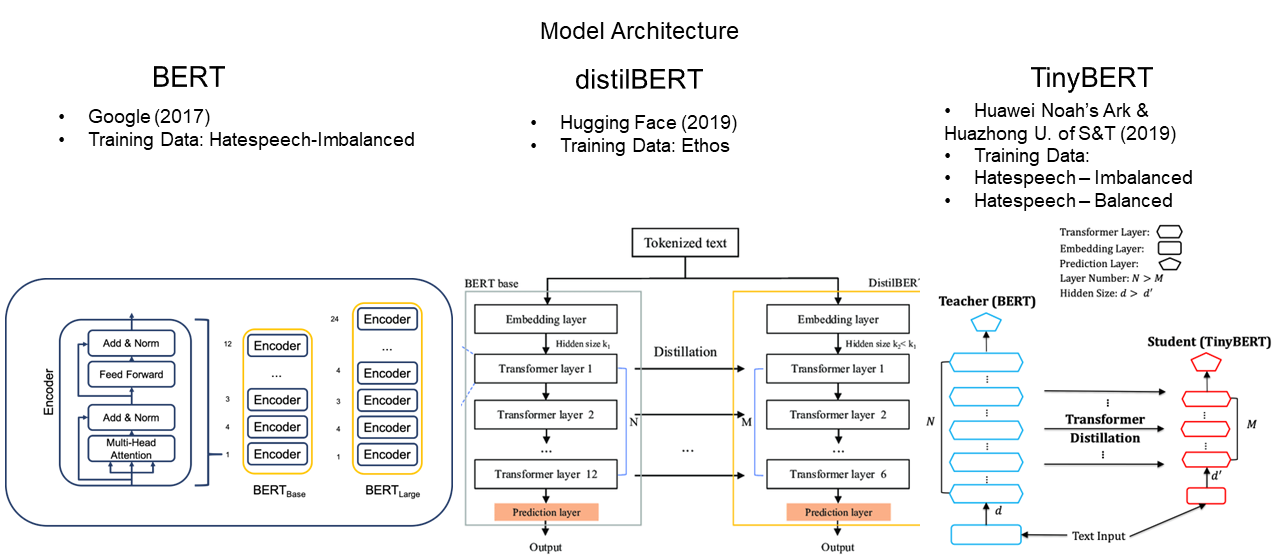
\includegraphics[scale = .5]{Slide1d.PNG}
    \caption*{BERT Source:\href{https://humboldt-wi.github.io/blog/img/seminar/bert/bert_architecture.png}{Bidirectional Encoder Representations from Transformers (BERT)}}
    \caption*{DistilBERT Source:\href{https://www.researchgate.net/profile/Alhassan-Mabrouk/publication/358239462/figure/fig2/AS:1120931644747777@1644262338087/The-DistilBERT-model-architecture-and-components.png}{Improving Crisis Events Detection Using DistilBERT with Hunger Games Search Algorithm}}
    \caption*{TinyBERT Source:\href{https://user-images.githubusercontent.com/38907104/90865208-fe72ee80-e3cc-11ea-869a-984330992d2f.png}{TinyBERT: Distilling BERT for Natural Language Understanding Number 22}}
\end{figure}
\begin{figure} [ht!]
    \centering
    \caption{Data flow for the project's three tested models}
    \label{fig:flow}
    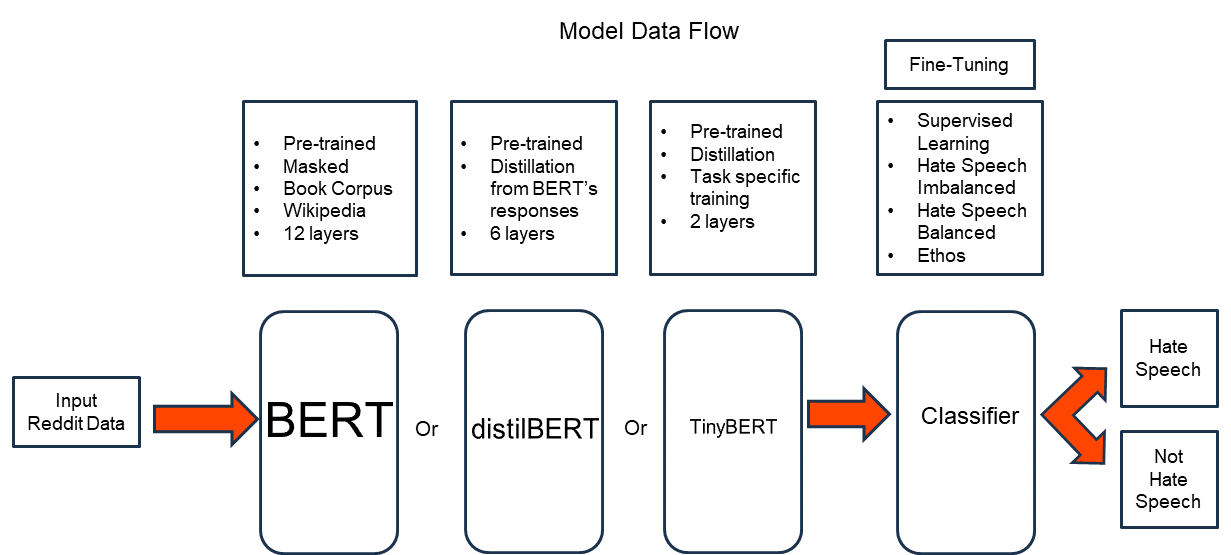
\includegraphics[scale = 0.5]{Slide2c.PNG}
    \caption*{Source: Author Graphic} 
    \caption*{Idea: \href{https://jalammar.github.io/images/BERT-classification-spam.png}{The Illustrated BERT, ELMo, and co. (How NLP Cracked Transfer Learning)}}
\end{figure}
\begin{figure} [ht!]
    \centering
    \caption{Histograms comparing model hate speech predictions before and after the Reddit policy change.}
    \label{fig:histogram}
    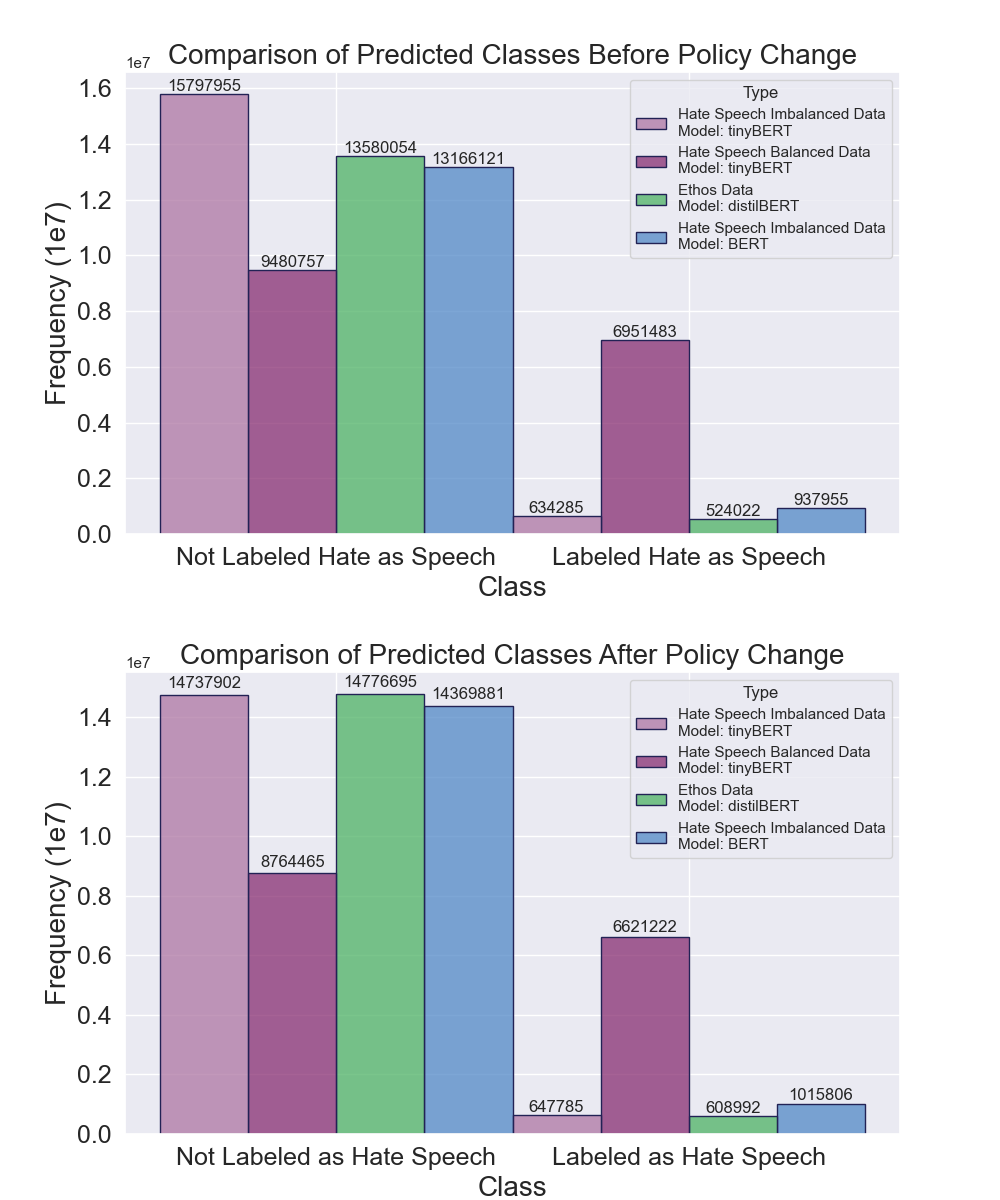
\includegraphics[scale = .5]{combined_histogram.png}
    \caption*{Source: Author Graphic}
\end{figure}
\clearpage
\begin{figure} [ht!]
    \centering
    \caption{Top 10 subreddits by predictions labeled as hate speech by model (before and after Reddit policy change).}
    \label{fig:top10}
    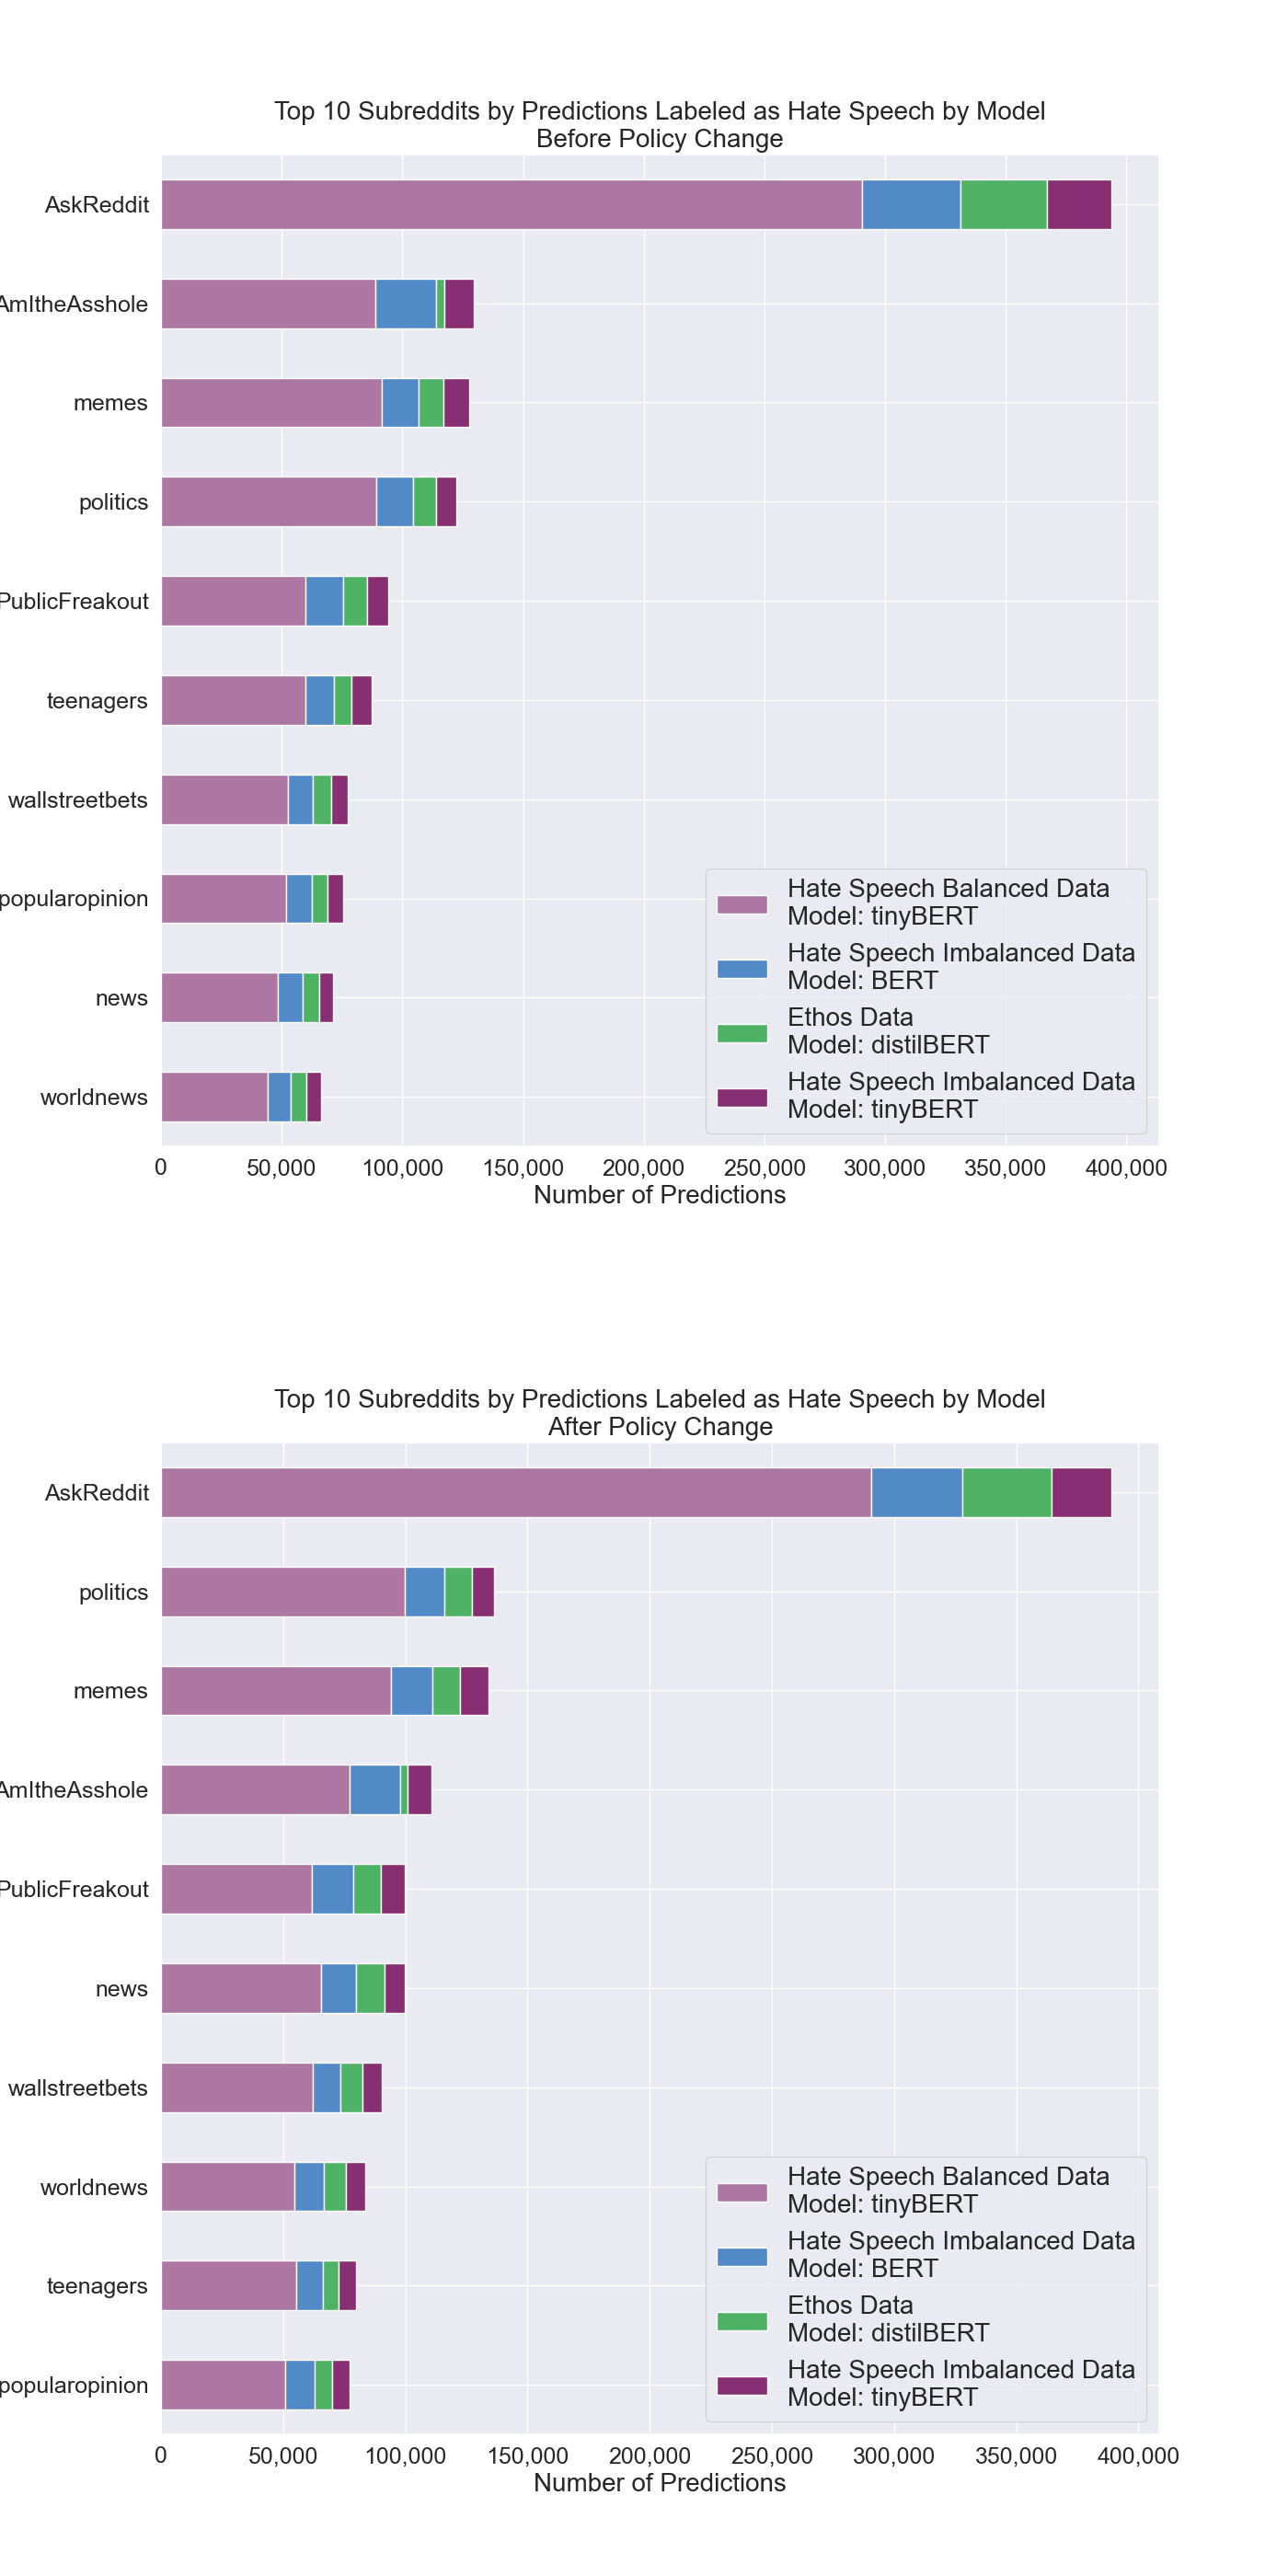
\includegraphics[scale = .25]{combined_top10.png}
    \caption*{Source: Author Graphic}
\end{figure}
\begin{figure}
    \centering
    \caption{Model agreements identified as hate speech in all test data.}
    \label{fig:agreement}
    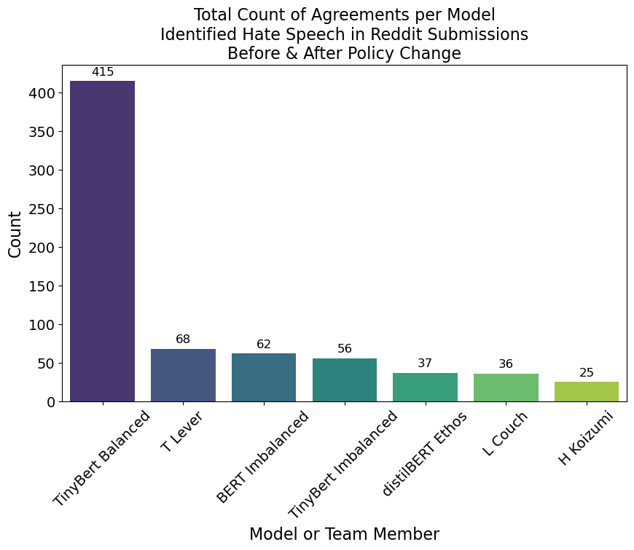
\includegraphics[scale=.7]{ModelTeam1.png}
    \caption*{Source: Author Graphic}
\end{figure}
\begin{figure}
    \centering
    \caption{Co-occurrence matrix of hate speech predictions by model and team member.}
    \label{fig:matrix}
    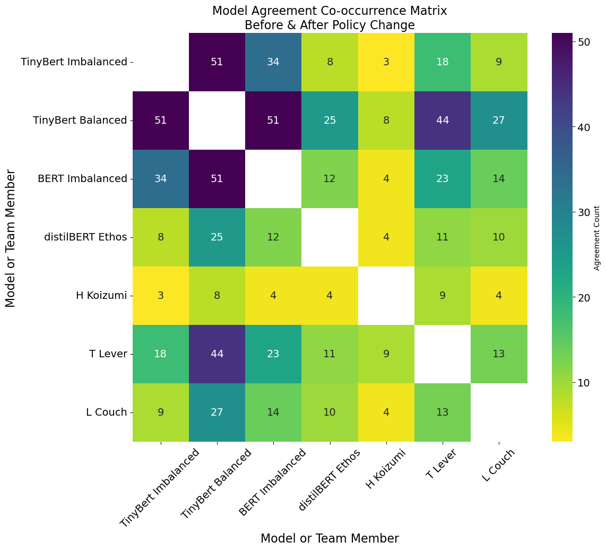
\includegraphics[scale=.7]{ModelTeam2.png}
    \caption*{Source: Author Graphic}
\end{figure}
\end{document}
\includegraphics{universe}